\documentclass{article}
\usepackage[utf8]{inputenc}

% inizia a copiare qua
\usepackage{ dsfont }
\usepackage{ amssymb }
%\usepackage{cases}
\usepackage{geometry}
 \geometry{
 a4paper,
 total={180mm,280mm},
 left=15mm,
 top=5mm,
 }
\usepackage{stackengine}
\usepackage{amsmath} 
\usepackage{mathtools}
\newcommand\ubar[1]{\stackunder[1.2pt]{$#1$}{\rule{.8ex}{.075ex}}}
\usepackage{graphicx}
\usepackage{wrapfig}
\graphicspath{ {./immagini/} }

\newcommand{\smat}{psmallmatrix}
\newcommand{\im}[2]{
\begin{center}
\includegraphics[width=#1\textwidth]{#2}
\end{center}
}

\newcommand{\ims}[3]{
\begin{center}
\includegraphics[width=#1\textwidth]{#2}
\includegraphics[width=#1\textwidth]{#3}
\end{center}
}

\newcommand{\R}{\mathds{R}}
\newcommand{\N}{\mathds{N}}
\newcommand{\C}{\mathds{C}}

\newcommand{\Index}{
\newpage
\renewcommand*\contentsname{Indice}
\tableofcontents
}


\title{Geometria 1}
\author{Luca Vettore}
\date{March 2022}

\begin{document}

\maketitle

\section{Relazioni}
Siano A e B insiemi, è detta relazione tra A e B un insieme $R\subseteq A\times B$. Sia $(a,b)\in R$, si dice che a è in relazione con b e si denota aRb.\\
Se $R\subseteq A\times A$, si dice che R è relazione in A.\\
Una relazione in un insieme A si dice di equivalenza se:
\begin{itemize}
    \item $\forall a\in A$ aRa (riflessività)
    \item $\forall a,b\in A$ aRb $\Leftrightarrow$ bRa (simmetria)
    \item $\forall a,b,c\in A$ aRb e bRc $\Rightarrow$ aRc (transitività)
\end{itemize}
Sia $R\subseteq A\times A$ una relazione di equivalenza, si dice classe di equivalenza l'insieme $[a]_R=\{\forall b\in A: bRa\}$ ($aRb\Leftrightarrow[a]_R=[b]_R$).\\
L'insieme delle classi di equivalenza si dice insieme quoziente e si denota $A/R=\{[a]_R;a\in a\}$ ("insieme di A modulo R").\\\\
Sia $A=\mathds{Z}\times(\mathds{Z}\setminus\{0\})$, sia $R\subseteq A\times A:$ $(a,b)R(c,d)\Leftrightarrow ad=bc$, allora $\mathds{Q}=A/R$.

\subsection{Classi modulo}
Siano $a,b\in\mathds{Z}$ e $n\in\mathds{N}$, si dice che a è congruo a b modulo n e si denota $a\sim b\Leftrightarrow\exists k\in\mathds{Z}:a-b=k\cdot n$.\\
$\sim$ è relazione di equivalenza.
L'insieme $\mathds{Z}/\sim=\mathds{Z}_n$ è detto insieme delle classi modulo n.\\
L'insieme $\mathds{Z}_2$ contiene due classi: $[0]_\sim=\{...,0,2,4,..\}$ e $[1]_\sim=\{...,1,3,5,..\}$.\\
L'insieme $\mathds{Z}_3$ contiene 3 classi ...\\
L'insieme $\mathds{Z}_n$ contiene n classi: $[0]_\sim,...,[n-1]_\sim$.

\section{Strutture algebriche}
\subsection{Operazioni}
Sia A un insieme. Un'operazione è un'applicazione $*:A\times A\rightarrow A$.\\
In $\mathds{Z}$ sono operazioni +,-,$\cdot$, non lo è : ($2:3\notin\mathds{Z}$).\\
In $\mathds{Z}_n$ si possono definire:\begin{itemize}
    \item +: $[a]_n+[b]_n=[a+b]_n$
    \item $\cdot:$ $[a]_n\cdot[b]_n=[a\cdot b]_n$
\end{itemize}
Queste operazioni sono indipendente dai rappresentanti della stessa classe scelti ($a\sim a', b\sim b'\Rightarrow a\cdot b\sim a'\cdot b'$).\\\\
Una struttura algebrica è un insieme dotato di operazioni che soddisfano determinate condizioni.

\subsection{Gruppi}
Un gruppo (G,*) è una struttura algebrica dotata di un operazione tale che:
\begin{enumerate}
    \item $\forall x,y\in G$ $(x*y)*z=x*(y*z)$ (associatività)
    \item $\exists e\in G:$ $\forall x\in G$ $e*x=x*e=x$ (esistenza elemento neutro)
    \item $\forall x\in G$ $\exists\bar{x}:$ $x*\bar{x}=x*\bar{x}=e$ (esistenza inverso)
\end{enumerate}
Un gruppo (G,*) è detto abeliano se: 4. $\forall x,y\in G$ $x*y=y*x$.\\
Una struttura che verifica 1 e 2 è detta monoide.\\\\
$(\mathds{Z},+), (\mathds{Q},+), (\mathds{Z}_n, +)$ sono gruppi abeliani.\\
$(\mathds{Z},\cdot), (\mathds{Q},\cdot), (\mathds{Z}_n, \cdot)$ non sono gruppi.\\
$(\mathds{Q}\setminus\{0\},\cdot)$ è un gruppo.\\\\
Sia (G,*) un gruppo, esso ha delle proprietà fondamentali:
\begin{itemize}
    \item L'elemento neutro è unico
    \item $\forall x\in G$ $\bar{x}$ è unico
    \item $x*y=x*z\Rightarrow y=z$ e $x*y=z*y\Rightarrow x=z$ (Leggi di cancellazione)
    \item $\overline{(x*y)}=\bar{x}*\bar{y}$
    \item $\overline{(\bar{x})}=x$
\end{itemize}
In un gruppo $(G,*)$ è possibile definire le potenze di $x\in G$ come operazioni ripetute di x con se stesso ($x^n=x*...*x$ per n volte). Le potenze godono delle usuali proprietà.

\subsection{Anelli}
Un anello $(A,+,*)$ è una struttura algebrica dotata di 2 operazioni tali che:
\begin{itemize}
    \item $(A,+)$ sia un gruppo abeliano
    \item * sia associativo ($c*(a*b)=a*(b*c)$)
    \item + e * siano distributive ($a*(b+c)=a*b+a*c$)
\end{itemize}
$(\mathds{Z},+,*);(\mathds{Q},+,*);(\mathds{Z}_n,+,*);(\mathds{R},+,*)$ sono anelli.\\\\
Un anello è detto commutativo se * è commutativo.\\\\
In $(A,+,*)$ $x\in A$ è detto divisore dello zero se $\exists b\in A: a*b=0_A$.\\
In $(\mathds{Z}_6,+,*)$ $[2],[3],[4]$ sono divisori dello zero.

\subsection{Campi}
Un anello $(K,+,*)$ è detto campo se $(K^*,*)$ è un gruppo abeliano.\\
$(\mathds{Z}_n,+,*)$ è un campo per n primo.

\subsection{Il campo complesso}
Sia $\mathds{C}=\mathds{R}\times\mathds{R}$. Rappresentiamo un elemento $z\in\mathds{C}$ come $z=a+i\cdot b$, con $a,b\in\mathds{R}$.\\
$a=Re(z)$ è detto parte reale e $b=Im(z)$ è detto parte immaginaria.\\\\
Definiamo due operazioni utilizzando le operazioni in $(\mathds{R},+_\mathds{R},*_\mathds{R})$
\begin{itemize}
    \item $+_\mathds{C}:\mathds{C}\times\mathds{C}\rightarrow\mathds{C}$: $(a+ib,c+id)\rightarrow(a+_\mathds{R}c)+(b+_\mathds{R}d)i$
    \item $*_\mathds{C}:\mathds{C}\times\mathds{C}\rightarrow\mathds{C}$: $(a+ib,c+id)\rightarrow(a*_\mathds{R}c-_\mathds{R}b*_\mathds{R}d)+(a*_\mathds{R}d+_\mathds{R}b*_\mathds{R}c)i$
\end{itemize}
$(\mathds{C},+_\mathds{C},*_\mathds{C})$ è un campo ed è chiamato campo complesso.\\\\
Esiste una corrispondenza tra gli elementi di $\mathds{R}$ e di $\mathds{C}$: $\forall r\in\mathds{R}$ $\exists z\in\mathds{C}:$ Re(z)=r e Im(z)=0.\\\\
Posto $i=0+1i$, $i^2=i*i=-1+0i$. Data questa eguaglianza il prodotto in $\mathds{C}$ segue le regole di un prodotto tra polinomi in i in $\mathds{R}$.\\\\
Un elemento di z è detto immaginario puro se $Re(z)=0$ o reale puro se $Im(z)=0$.\\\\
Sia $z=a+bi$ un numero complesso, il suo coniugato è definito come $\bar{z}=a-bi$.\\\\
Un numero complesso può essere rappresentato come un vettore su un piano $\mathds{R}\times\mathds{R}$ noto come piano di Angart-Gauss.
In questo modo l'operazione di somma tra numeri complessi assume il significato di somma di vettori.
\begin{center}
    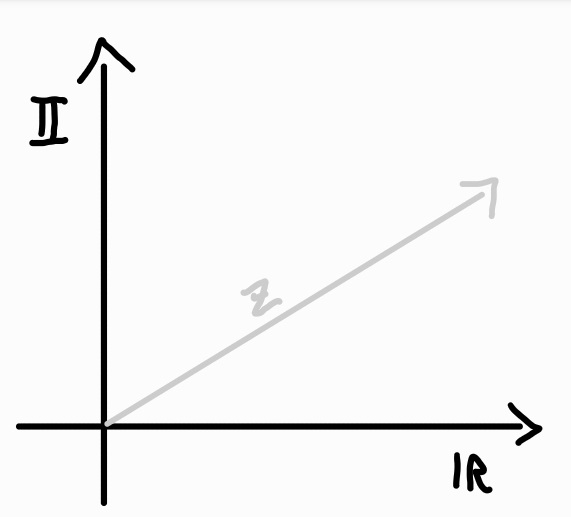
\includegraphics[width=0.2\textwidth]{im1}
    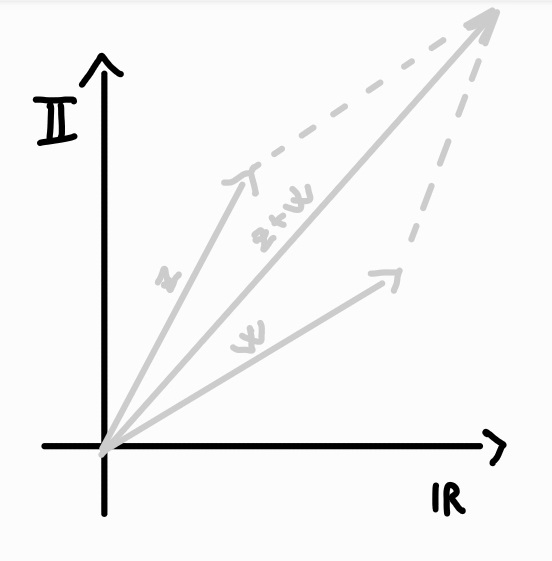
\includegraphics[width=0.175\textwidth]{im2}
\end{center}
Definiamo l'argomento $\theta$ come l'angolo compreso tra l'asse reale e il vettore z (in senso antiorario), z può quindi essere espresso come $z=a+bi=\rho(cos(\theta)+isin(\theta))$, dove $\rho=\sqrt{a^2+b^2}$ è il modulo di z ($tan(\theta)=\frac{b}{a}$ con $a\neq 0$, $a=\rho cos(\theta)$, $b=\rho sin(\theta)$). Questa forma è nota come forma trigonometrica\\
Il prodotto di numeri complessi si può quindi scrivere come $z=\rho(cos(\theta)+sin(\theta)i),w=\eta(cos(\psi)+sin(\psi)i)$ $z\cdot w=\rho\cdot\eta(cos(\theta+\psi)+sin(\theta+\psi)i)$
\begin{center}
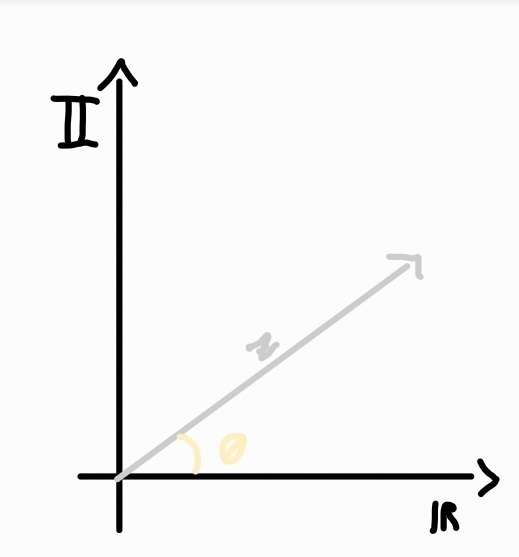
\includegraphics[width=0.2\textwidth]{im3}
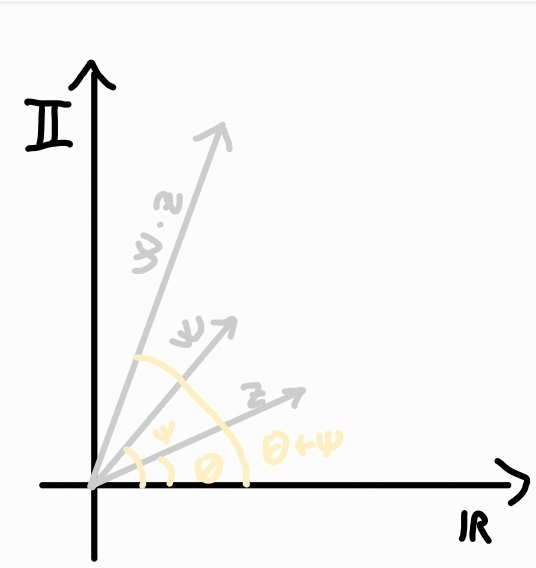
\includegraphics[width=0.2\textwidth]{im4}
\end{center}
Ponendo $z^{-1}=\frac{1}{\rho}(cos(-\theta)+sin(-\theta)i)$ è possibile definire il rapporto in $\mathds{C}$ come $z/w=z*w^{-1}$\\\\
Le potenze in $\mathds{C}$ sono definite (per $n\geq1)$ come prodotti ripetuti: $z^n=z*...*z$ n volte (formula di de Moivre).\\\\
Siano $z,w\in\mathds{C}$, $z=\rho(cos(\theta)+sin(\theta)i),w=\eta(cos(\psi)+sin(\psi)i)$, si dice che z è radice n-esima di w se $z^n=w$, cioè $\rho^n=\eta$ e $\theta=\frac{\psi}{n}+\frac{2k\pi}{n}$ con $k\in\mathds{N}$.\\
Sia $k'\sim k$ (mod n), allora $k'=k+rn$ con $r\in\mathds{N}\Rightarrow\frac{\psi}{n}+\frac{2k'\pi}{n}=\frac{\psi}{n}+\frac{2k\pi}{n}+\frac{2\pi rn}{n}\sim \frac{\psi}{n}+\frac{2k\pi}{n}$ (mod n), quindi le radici distinte vanno ricercate nei valori $0\leq k<n$.\\
In $\mathds{C}$ un numero ha n radici n-esime.\\\\
Le radici n-esime di $z=\rho(cos(\theta)+sin(\theta)i)$ su un piano di Angart-Gauss sono disposte su una circonferenza con centro nell'origine e raggio $\sqrt[n]{\rho}$.\\
Nel caso di $w=1+0i$:
\begin{center}
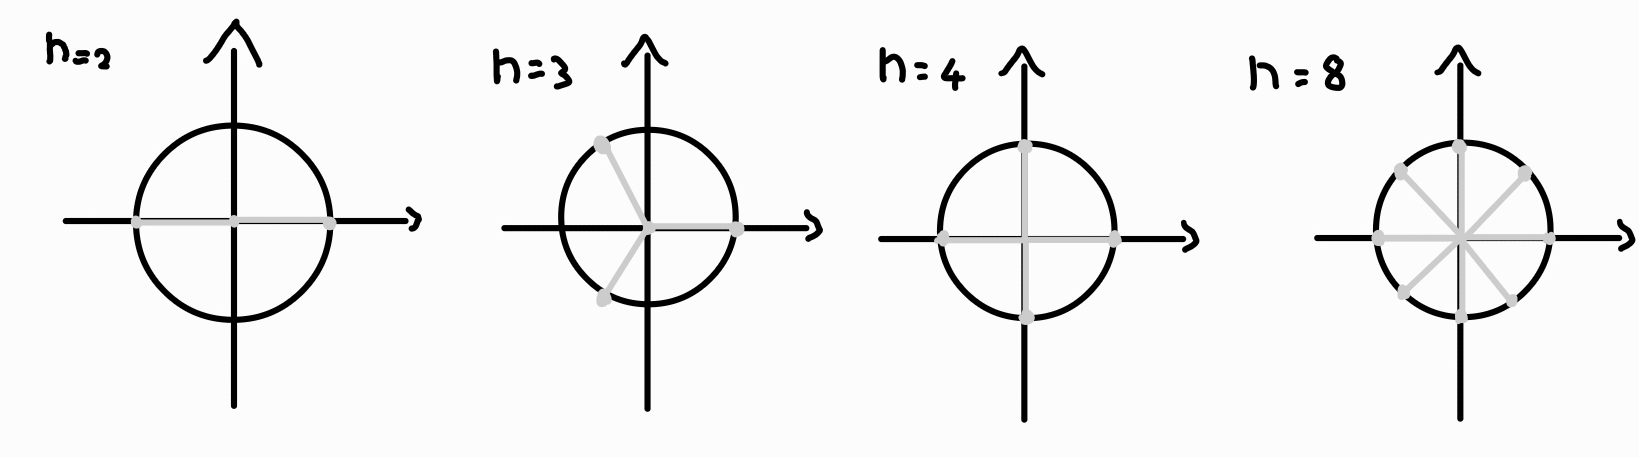
\includegraphics[width=0.9\textwidth]{im5}
\end{center}


\subsubsection{Teorema fondamentale dell'algebra}
Il campo $\C$ è algebricamente chiuso, cioè ogni polinomio $p(z)\in\C[z]$ di grado $\geq1$ si può scomporre come $p(z)=a(z-\alpha_1)...(z-\alpha_d)$, dove $\alpha_n$ è radice di $p(x)$.\\\\
Sia $p(z)\in\C[z]$ con tutti i coefficienti reali, allora se $\alpha\in\C$ è radice, anche $\bar{\alpha}$ è radice del polinomio e $p(\bar{z})=\bar{p(z)}$.\\\


\section{Matrici}
Una matrice di dimensione m$\times$n o a m righe e n colonne è una tabella del tipo $\begin{\smat} a_{11} & a_{22} & ... & a_{1n} \\ .. & .. & .. & ... \\ a_{1m} & ... & ... & a_{mn} \end{\smat}$\\
L'insieme delle matrici di dimensioni m*n si denota con $Mat_{mn}(K)$, dove k è il campo a cui apartengono i termini della matrice.\\
Tra matrici delle stesse dimensioni si definisce la somma, come somma elemento per elemento, e il prodotto per scalare, come prodotto di ogni elemento per lo scalare.\\
Una matrice formata da una sola colonna è detta vettore.
\subsection{Prodotto righe per colonne}
Siano $A\in Mat_{m,n}$ e $B\in Mat_{s,p}$, A e B sono dette conformabili se $n=s$. In tal caso si può definire il prodotto tra matrici, come la matrice che ha come elementi $c_{ij}:=a_{i1}b_{1j}+a_{i2}b_{2j}+...+a_{in}b_{nj}$. Questa operazione è anche nota come prodotto righe per colonne.\\\\
Il prodotto tra matrici ha alcune proprietà:
\begin{itemize}
    \item $A*(B+C)=A*B+A*C$
    \item $(A+B)*C=A*C+B*C$
    \item $(A*B)*C=A*(B*C)$
    \item $\lambda(A*B)=(\lambda A)*B=A*(\lambda B)$
\end{itemize}

Data una matrice A, la sua trasposta $A^T$ è la matrice che ha per colonne le righe di A.\\
L'elemento neutro rispetto al prodotto tra matrici è la matrice identità, composta di 1 sulla diagonale.

\subsection{Matrici e sistemi lineari}
Un sistema di equazioni lineari può essere rappresentato come $A*x=b$, dove A  una matrice contenente i coefficienti, x un vettore contenente le incognite e b un vettore formato dai termini noti.\\
Una soluzione del sistema è un vettore $\Tilde{x}$ tale che $A*\Tilde{x}=b$.\\
Un sistema si dice:
\begin{itemize}
    \item impossibile: se non ammette soluzioni
    \item determinato: se ammette una e una sola soluzione
    \item indeterminato: se ha più di una soluzione
\end{itemize}
Due sistemi lineari sono equivalenti se hanno le stesse soluzioni.\\\\
Il metodo di Gauss è un metodo che permette di trovare la soluzione di un sistema lineare. Il metodo consiste nel ridurre il sistema lineare in un sistema a scalini applicando delle operazioni che lo trasformino in uno equivalente. Un sistema a scalini è strutturato così: $\begin{\smat} *&*&*&*&*\\0&*&*&*\\0&0&*&*&*\\... \end{\smat}$, ogni riga ha almeno uno zero più della precedente prima di un valore non nullo.\\\\
Le operazioni che mantengono le soluzioni di un sistema sono:
\begin{itemize}
    \item Scambio di righe fra loro
    \item Moltiplicazione di una riga per costante non nulla
    \item Somma di una riga al multiplo di un altra
\end{itemize}

\subsection{Rango}
Il procedimento di Gauss può essere applicato a una qualsiasi matrice. Il numero di righe non nulle di una matrice ridotta a scalini è detto rango o caratteristica della matrice.\\\\
\textbf{Teorema di Rouché-Capelli}\\
Il sistema lineare $Ax=b$ se ha soluzioni, ne ha $\infty^{n-r}$, dove n è il numero di righe e r il rango di A.

\section{Spazi vettoriali}
Sia K un campo, un insieme V si dice spazio vettoriale sul campo K se è dotato di due operazioni $+:V\times V\rightarrow V$ e $\cdot:K\times V\rightarrow V$ con le seguenti proprietà:
\begin{itemize}
    \item $(V,+)$ è un gruppo abeliano
    \item $\forall \lambda,\mu\in K,$ $\forall u,v\in V$ si ha:
    \begin{itemize}
        \item $(\lambda+\mu)u=\lambda u + \mu u$
        \item $(\lambda*\mu)u=\lambda*(\mu*u)$
        \item $\lambda(u+v)=\lambda u + \lambda v$
        \item $1_K*u=u$
    \end{itemize}
\end{itemize}
Dati $\lambda_1,...,\lambda_n\in K$ e $v_1,...,v_n\in V$, $\lambda_1v_1+...+\lambda_nv_n$ è detta combinazione lineare di $v_1,...,v_n$ con coefficienti $\lambda_1,...,\lambda_n$.\\\\
Uno spazio vettoriale generico ha le seguenti proprietà:
\begin{itemize}
    \item le proprietà di $(V,+)$ abeliano
    \item $\forall v$ $0*v=0$
    \item $\forall \lambda\in K$ $\lambda*0=0$
    \item $\forall v$, $\forall \lambda\in K$ $-(\lambda*v)=(-\lambda))*v$
    \item $\lambda*v=0\Rightarrow$ $\lambda=0\vee v=0$
\end{itemize}

\subsection{Sottospazi}
Dato uno spazio vettoriale V, si dice sottospazio di V un insieme $U\subseteq V$ tale che:
\begin{itemize}
    \item $\forall u,v\in U$ $(u+v)\in U$
    \item $\forall \lambda\in K$ $\forall u\in U$ $(\lambda u)\in U$
    \item $0\in U$
\end{itemize}
Le prime due proprietà dicono che un sottospazio è chiuso rispetto alle combinazioni lineari.\\\\
Sia V uno spazio vettoriale sul campo K e siano U e W sottospazi di V, allora l'insieme $U\cap W$ è sottospazio di V, mentre l'insieme $W\cup U$ può non esserlo.\\
Si definisce quindi il sottospazio somma di W e U come $U+W=\{v\in V|\exists u\in U, \exists w\in W: v=w+u\}$. Nel caso in cui $U\cap W=\emptyset$ la somma è detta diretta.\\\\
\textbf{Teorema}\\
La somma di U e W è diretta se e solo se ogni $v\in (U+W)$ si scrive in uno e un solo modo come somma di $u\in U$ e $w\in W$.

\section{Generatori e basi}
Sia V spazio vettoriale sul campo K. Sia $S={s_\alpha}_{\alpha\in A}\subseteq V$ e $S\neq\emptyset$, si dice sottospazio generato da S o span di s, l'insieme $<S>=<s_\alpha>_{\alpha\in A}=\{v\in V|\exists \lambda_1,...\lambda_n, \exists s_{\alpha_1},...,s_{\alpha_n}: v=\lambda_1 s_{\alpha_1}+...+\lambda_n s_{\alpha_n}\}$.\\
Gli elementi di S sono detti generatori di $<S>$.\\\\
$<S>$ è un sottospazio di V.\\
Sia $U\subseteq V$ e $\exists S_\{s_1,...,s_k\}: U=<S>$, allora U si dice finitamente generato.

\subsection{Dipendenza lineare}
Sia V spazio vettoriale su K. Sia $S=\{s_\alpha\}_{\alpha\in A}\subseteq V$, $S\neq\emptyset$.\\
Si dice che gli elementi di S sono linearmente dipendenti se $\exists \lambda_1,...,\lambda_n\in K$ e $s_{\alpha_1},...,s_{\alpha_n}\in S$ tali che $(\lambda_1,...,\lambda_n)\neq(0,...,0)$ e $\lambda_1 s_{\alpha_1}+...+\lambda_n s_{\alpha_n}=0$.\\
Se gli elementi si S non sono linearmente dipendenti, allora sono linearmente indipendenti.\\\\
La dipendenza lineare ha le seguenti proprietà:
\begin{itemize}
    \item $S\neq\emptyset$, $S\subseteq T\subseteq V$, S l.d $\Rightarrow$ T l.d
    \item $S=\{v\}$, S l.d $\Leftrightarrow v=0$
    \item $0\in S\Rightarrow$ S l.d
    \item $S=\{v_1,v_2\}$, S l.d $\Leftrightarrow$ uno è multiplo dell'altro
    \item $S=\{v_1,...,v_n\}$, S l.d $\Leftrightarrow$ uno è combinazione lineare degli altri
    \item $\lambda_1 v_1+...+\lambda_n v_n=0$, $\lambda_1\neq 0\Rightarrow v_1\in <v_2,...,v_n>$
\end{itemize}

\subsection{Basi}
Un sottoinsieme $B\subset V$ si dice base di V se:
\begin{itemize}
    \item $<B>=V$
    \item B è linearmente indipendente
\end{itemize}
\textbf{Teorema}\\
$B\subset V$ è base di V se e solo se ogni elemento di v può essere scritto in uno e un solo modo come combinazione lineare degli elementi di B.\\\\
\textbf{Teorema}\\
Sia $V\neq\emptyset$ uno spazio vettoriale su K e sia $V=<v_1,...,v_n>$, allora $\{v_1,...,v_n\}$ contiene una base di V.\\\\
Un insieme $\{v_1,...,v_k\}\subseteq V$ si dice insieme massimale di linearmente indipendenti se:
\begin{itemize}
    \item $\{v_1,...,v_k\}$ è l.i.
    \item $\forall v\in V$ $\{v_1,...,v_k,v\}$ è l.d.
\end{itemize}
\textbf{Teorema}\\
Sia $\{v_1,...,v_k\}$ un insieme massimale di linearmente indipendenti, allora $\{v_1,...,v_k\}$ è una base.\\\\

Un insieme $\{v_1,...,v_k\}\subseteq V$ si dice insieme minimale di generatori se:
\begin{itemize}
    \item $<v_1,...,v_k>=V$
    \item $\forall i=1,...,k$ $\{v_1,...,v_k\}\setminus \{v_i\}$ non genera V
\end{itemize}
\textbf{Teorema}\\
Sia $\{v_1,...,v_k\}\subseteq V$ un insieme minimale di generatori, allora $\{v_1,...,v_k\}\subseteq V$ è una base.\\\\
\textbf{Teorema: Equicardinalità delle basi}\\
Sia V uno spazio vettoriale che ha una base con n vettori, allora qualsiasi insieme di $m>n$ vettori è linearmente dipendente\\\\
\textbf{Corollario}\\
Sia V uno spazio vettoriale e siano A e B due sue basi, allora A e B hanno lo stesso numero di elementi.

\subsection{Dimensioni di uno spazio vettoriale}
Sia V uno spazio vettoriale su K.
\begin{itemize}
    \item Se $V=\{0\}$ si dice che V ha dimensione nulla ($dimV=0$).
    \item Se V non è finitamente generato si dice che V ha dimensione infinita ($dimV=\infty$).
    \item Se $V\neq\{0\}$ ed è generato da una base $B=\{b_1,...,b_n\}$, allora V ha dimensione k ($dimV=n$).
\end{itemize}
\textbf{Teorema}\\
Sia V spazio vettoriale e $dimV=n$, allora $\{v_1,...,v_n\}$ l.i. $\Rightarrow \{v_1,...,v_n\}$ base\\\\
\textbf{Teorema}\\
V sp. vett., dimV=n, allora $<v_1,...,v_n>=V\Rightarrow\{v_1,...,v_n\}$ base.\\\\
\textbf{Teorema}\\
V sp. vett., dimV=n e $U\subseteq V$ sottospazio, allora U è finitamente generato e $dimU\leq dimV$.\\
Inoltre, $dimU=dimV\Leftrightarrow U=V$\\\\
\textbf{Teorema}\\
Sia V sp. vett. con $dimV=n>0$, allora presi r vettori l.i. $w_1,...,w_r\in V$ $\exists w_{r+1},...,w_n$ tali che $\{w_1,...,w_r,w_{r+1},...,w_n\}$ sia base.\\\\
\textbf{Teorema: formula di Grassman}\\
Sia V uno spazio vettoriale su K e siano X e Y sottospazi, allora $X\cap Y$ e $X+Y$ sono finitamente generati e $dimX+dimY=dimX\cap Y+dim(X+Y)$

\section{Applicazioni lineari}
Siano W e V due spazi vettoriali sullo stesso campo e sia $F:V\rightarrow W$ una funzione. Si dice che f è lineare su K se:
\begin{itemize}
    \item $\forall u,v\in V$ $f(u+v)=f(u)+f(v)$ (additività)
    \item $\forall\lambda\in K, \forall u\in V$ $f(\lambda u)=\lambda f(u)$ (omogeneità)
\end{itemize}
Se f è lineare, allora mantiene le combinazioni lineari.\\
Se f è lineare, allora $f(0_V)=0_W$.\\
Una funzione lineare e biunivoca è detta isomorfismo\\\\
\textbf{Teorema}\\
Se $f:V\rightarrow W$ e $g:W\rightarrow Z$ sono lineari, allora $(g\circ f):V\rightarrow Z$ è lineare.\\
Se $f:V\rightarrow W$ è lineare e biunivoca, allora $f^{-1}:W\rightarrow V$ è lineare.\\\\
\textbf{Teorema: esistenza e unicità}\\
Siano V e W spazi vettoriali, con V finitamente generato. Sia $B=\{b_1,...,b_n\}$ una base di V e siano $w_1,...,w_n\in W$ qualsiasi, allora $\exists!$ $f:V\rightarrow W$ lineare tale che $f(b_1)=w_1,...,f(b_n)=w_n$\\\\
Lo spazio $L(V,W)$ delle applicazioni lineari da V a W è vettoriale rispetto a:
\begin{itemize}
    \item $+:L(V,W)\times L(V,W)\rightarrow L(V,W)$\\
    $(f(x),g(x))\rightarrow (f+g)(x)=f(x)+g(x)$
    \item $*:K\times L(V,W)\rightarrow L(V,W)$\\
    $(\lambda,f(x))\rightarrow (\lambda f)(x)=\lambda*f(x)$
\end{itemize}
\subsection{Nucleo e immagine}
Sia $f:V\rightarrow W$ lineare.\\
Si chiama nucleo o kernel di f l'insieme $ker(f)=\{v\in V|f(v)=0_v)\}$.\\
Si chiama immagine di f l'insieme $Im(f)=\{w\in W|\exists v\in V: f(v)=w\}$\\
Nucleo e immagine sono sottospazi di V.\\\\
\textbf{Teorema: nullità + rango}\\
Siano V e W spazi vettoriali su K finitamente generati e sia $f:V\rightarrow W$ lineare, allora $ker(f)$ e $Im(f)$ sono finitamente generati e vale:
$$dimV=dim(ker(f))+dim(Im(f)) $$

\subsection{Iniettività e suriettività}
Siano W e V spazi vettoriali su K finitamente generati.\\\\
\textbf{Teorema: iniettività}\\
Sia $f:V\rightarrow W$ lineare, allora sono equivalenti
\begin{itemize}
    \item f è iniettiva
    \item $ker(f)=\{0\}$
    \item se $v_1,...,v_k$ sono l.i. $\Rightarrow$ $f(v_1),...,f(v_k)$ l.i.
\end{itemize}
\textbf{Teorema: suriettività}\\
Sia $f:V\rightarrow W$ lineare, allora sono equivalenti
\begin{itemize}
    \item f è suriettiva
    \item $dim(Im(f))=dim(W)$
    \item se $<v_1,...,v_k>=V\Rightarrow<f(v_1),...,f(v_k)>=W$
\end{itemize}
In ogni caso vale $<v_1,...,v_k>=V\Rightarrow<f(v_1),...,f(v_k)>=Im(f)$\\\\
\textbf{Corollario}\\
Sia $f:V\rightarrow W$, allora f è isomorfismo $\Leftrightarrow$ f manda una base di V in una base di W

\subsection{Definizioni}
Sia $f:V\rightarrow W$ lineare:
\begin{itemize}
    \item se f è biunivoca è detta isomorfismo
    \item se $V=W$ è detta endomorfismo o operatore
    \item se $V=W$ e f è biunivoca è detta automorfismo
\end{itemize}
Due spazi V e W sono detti isomorfi se $\exists f:V\rightarrow W$ isomorfismo e si indica $V\simeq W$.\\\\
\textbf{Teorema: spazi isomorfi}\\
$V\simeq W\Leftrightarrow dimV=dimW$
\textbf{Corollario}\\
V e W finitamente generati, allora:
\begin{itemize}
    \item $dimV>dimW\rightarrow\nexists f:V\rightarrow W$ iniettiva
    \item $dimV<dimW\rightarrow\nexists f:V\rightarrow W$ suriettiva
\end{itemize}

\subsection{Matrici rappresentative}

\subsection{Determinante}
[spostare sotto matrici?]\\
Una permutazione di n elementi è una funzione biunivoca $\sigma:[1,n]\cap\N\rightarrow[1,n]\cap\N$. Una permutazione si dice pari se è composta da un numero pari di scambi, altrimenti dispari.\\
Definito $\epsilon(\sigma)=$ $\begin{cases} +1\; se\; \epsilon\; pari\\ -1\; se\; \epsilon\; dispari \end{cases}$\\
Sia $A\in Mat_n(K)$, si definisce determinante lo scalare: $$detA=\Sigma_{\sigma}\epsilon(\sigma)\alpha_{1,\sigma(1)}*...*\alpha_{n,\sigma(n)}$$
Il determinante ha le seguenti proprietà:
\begin{itemize}
    \item $det(A)=det(A^t)$
    \item Scambiando righe o colonne tra loro cambia solo il segno del determinante
    \item Il determinante è lineare in ogni riga e colonna fissate le altre
    \item Il determinante dell'identità vale 1
    \item $det(A*B)=det(A)*det(B)$
    \item Le righe o colonne di A sono l.d $\Leftrightarrow det(A)=0$
    \item $det(\lambda A)=\lambda^n det(A)$
    \item A è invertibile $\Leftrightarrow det(A)\neq 0$
    \item Se A è invertibile, allora $det(A^-1)=\frac{1}{det(A)}$
\end{itemize}

\subsubsection{Teoremi di Laplace}
Sia $M\in Mat_n(K)$, si dice sottomatrice di M la matrice ottenuta eliminando un certo numero di righe e colonne da M.
Se N è sottomatrice quadrata di M, allora $det(N)$ è detto minore di M.\\
Il determinante della matrice $A_{ij}$ ottenuta eliminando la riga i e la colonna j si dice minore complementare di $\alpha_{ij}$.\\\\
Si dice cofattore o complemento algebrico il numero: $$ A_{ij}=(-1)^{i+j}det(M_{ij}) $$
La matrice $cof(A)$ composta dai cofattori degli elementi di A, viene detta matrice dei cofattori di A.\\\\
\textbf{Teorema: primo teorema di Laplace}\\
Per l i-esima riga: $$ detA=\alpha_{i1}A_{i1}+\alpha_{i2}A_{i2}+...+\alpha_{in}A_{in} $$
Per l j-esima colonna: $$ detA=\alpha_{1j}A_{1j}+\alpha_{2j}A_{2j}+...+\alpha_{nj}A_{nj} $$
\textbf{Teorema: secondo teorema di Laplace}\\
Per righe: se $i\neq j$ $$ detA=\alpha_{i1}A_{j1}+\alpha_{i2}A_{j2}+...+\alpha_{in}A_{jn} $$
Per colonne: se $i\neq j$ $$ detA=\alpha_{1i}A_{1j}+\alpha_{2i}A_{2j}+...+\alpha_{ni}A_{nj} $$
\textbf{Lemma}\\
$A*cof(A)^T=det(A)*I$\\\\
\textbf{Teorema}\\
Sia $A\in Mat_n(K)$ con $det(A)\neq0\Rightarrow\exists A^{-1}$ e $A^{-1}=\frac{1}{det(A)}(cof(A))^T$

\subsubsection{Formula di Cramer}
Sia $A\in Mat_n$ con $det(A)\neq0$ e sia $b\in K^n$.\\
Il sistema $Ax=b$ è detto sistema Crameriano e ha una e una sola soluzione che vale:
$x=\begin{psmallmatrix} x_i\\...\\...\\x_n \end{psmallmatrix}$ con
$$x_i=\frac{det(A^{(1)},...,A^{(i-1)},b,A^{(i+1)},...,A^{(n)})}{det(A)} $$

\subsection{Rango}
La nozione di rango può essere espressa in 4 modi equivalenti:
\begin{itemize}
    \item Caratteristica della matrice: il numero di righe non nulle della matrice ridotta con il metodo di Gauss
    \item Rango per colonne: la dimensione dello spazio generato dalle colonne della matrice
    \item Rango per righe: la dimensione dello spazio generato dalle righe
    \item Rango per minori: il massimo ordine di minore non nullo estratto dalla matrice
\end{itemize}

\section{Endomorfismi}
\subsection{Autovettori, autovalori e matrici diagonali}
Sia V uno spazio vettoriale su K finitamente generato.\\
Un vettore $v\in V$ tale che $f(v)\lambda v$ con $\lambda\in K$ è detto autovettore, mentre $\lambda$ è detto autovalore relativo a v.\\
Lo spazio $V\lambda(f)=\{v\in V|f(v)=\lambda v\}$ è detto autospazio di f relativo a $\lambda$ ed è un sottospazio di V.\\\\
Un endomorfismo f è detto diagonale se è presentata nella forma $M_B^B(f)=\begin{psmallmatrix} \lambda & 0 & 0 & ... \\ 0 & \lambda & 0 & ... \\ 0 & 0 & \lambda \end{psmallmatrix}$.\\
Se esiste una base di V tale per cui un endomorfismo risulti diagonale, allora è detto diagonalizzabile e la base è detta diagonalizzante.\\\\
La nozione di endomorfismo diagonale, diagonalizzabile, di autovettore e autovalore può essere estesa a matrici qualsiasi.\\\\
\textbf{Teorema}\\
Un endomorfismo è diagonalizzabile $\Leftrightarrow \exists$ una base composta dei suoi autovettori.\\\\
\textbf{Teorema}
Siano $\lambda_1,...,\lambda_n$ autovalori distinti di f endomorfismo, allora gli autovettori $v_1,...,v_n$ a loro associati sono linearmente indipendenti.\\\\
\textbf{Corollario}\\
Se f ha $n=dim(V)$ autovalori distinti, allora f è diagonalizzabile.\\\\
\textbf{Teorema: ricerca di autovalori}\\
$\lambda$ è autovalore di f $\Leftrightarrow det(A-\lambda Id)=0$, e in tal caso gli autovettori associati a $\lambda$ sono le soluzioni del sistema lineare $(A-\lambda Id)x=0$

\subsection{Polinomio caratteristico}
Sia $A\in Mat_n$, si dice polinomio caratteristico il polinomio $P_A(t)=det(A-t *Id)$.\\\\
Due matrici simili hanno lo stesso polinomio caratteristico e quindi stesso determinante (t=0). Le matrici che rappresentano lo stesso endomorfismo sono simili, per questo si può parlare di polinomio caratteristico o di determinante di un endomorfismo senza specificare in che base.\\\\
Il polinomio caratteristico di $A\in Mat_n$ ha le seguenti proprietà:
\begin{itemize}
    \item ha grado n
    \item ha coefficiente direttore (il coefficiente del termine di grado massimo) $(-1)^n$
    \item ha termine noto $P_A(0)=det(A)$
    \item ha come coefficiente di $t^{n-1}$ $(-1)^{n-1}(a_11+a_22+...+a_nn)=(-1)^{n-1} Tr(A)$
    \item ha come radici in K gli autovalori di A
\end{itemize}

\subsubsection{Molteplicità algebrica e geometrica}
Sia f un endomorfismo nello spazio vettoriale V su K e sia $\lambda\in K$ autovalore di f.\\
La molteplicità algebrica $m_a(\lambda)$ di $\lambda$ è la sua molteplicità come radice di $P_f(t)$.\\
La molteplicità geometrica $m_g(\lambda)$ di $\lambda$ è la dimensione dell'autospazio $V_\lambda(f)$.\\\\
\textbf{Teorema}\\
Sia $\lambda\in K$ autovalore di f, si ha che $1\leq m_g(\lambda)\leq m_a(\lambda)$\\\\
\textbf{Teorema: condizione sufficiente e necessaria di diagonalizzabilità}\\
Sia V spazio vettoriale su K ($dimV=n$) e sia f un endomorfismo su V, allora f è diagonalizzabile $\Leftrightarrow$ \begin{itemize}
    \item Tutte le radici di $P_f(t)$ sono in K
    \item $\forall \lambda$ autovalore di f si ha $m_a(\lambda)=m_g(\lambda)$
\end{itemize}

\section{Forme bilineari}
V spazio vettoriale su K, $dimV=n$.\\
Si dice forma bilineare un'applicazione lineare $\varphi:V\times V\rightarrow K$, tale che $\forall u,v,w\in V$, $\forall \alpha, \beta\in K$:
\begin{itemize}
    \item linearità a sinistra: $\varphi(\alpha v+\beta u, w)=\alpha\varphi(v,w)+\beta\varphi(u,w)$
    \item linearità a destra: $\varphi(u, \alpha v+\beta w)=\alpha\varphi(u,v)+\beta\varphi(u,w)$
\end{itemize}
Ogni forma bilineare può essere rappresentata da una matrice. Sia $A=\{a_1,...,a_n\}$ una base di V, è possibile ricavare la matrice rappresentativa di $\varphi$ su A come $ A_\varphi=(\alpha_{ij})=\varphi(a_i,a_j)$\\\\
Due matrici $A$ e $A'$ sono congruenti $\Leftrightarrow$ rappresentano la stessa forma bilineare in basi diverse.

\subsection{Tensori}
Si dice forma bilineare o tensore un'applicazione lineare $\varphi:V\times .... \times V\rightarrow K$ lineare in ciascuno dei suoi argomenti.\\
Una forma multilineare a n argomenti può essere rappresentata dall'analogo n dimensionale di una matrice.

\subsection{Forme bilineari simmeriche}
Una forma bilineare $\varphi:V\times V\rightarrow K$ si dice simmetrica se
$\forall u,v\in V$ $$\varphi(u,v)=\varphi(v,u)$$
Una forma bilineare è simmetrica se e solo se la sua matrice associata A verifica la proprietà $A=A^T$\\
Una forma bilineare si dice degenere se $\exists v\in V, v\neq0$ tale che $\forall w\in V$ $\varphi(v,w)=0$, in tal caso, la sua matrice associata è tale che $\exists x\neq0:$ $A\cdot x=0$\\\\
Sia $\varphi V\times V\rightarrow \R$ bilineare e simmetrica, $\varphi$ è detta definita positiva se:
\begin{itemize}
    \item $\forall v\in V$ $\varphi(v,v)\geq0$
    \item $\varphi(v,v)=0\Leftrightarrow v=0$
\end{itemize}
Una forma bilineare simmetrica definita positiva è detta prodotto scalare o prodotto interno e si indica $$\varphi(u,v)=<u,v>$$\\
Un prodotto scalare non è degenere.


\section{Spazi vettoriali euclidei}
Sia V uno spazio vettoriale si $\R$ , $dimV=n$.\\
Sia $\varphi$ un prodotto scalare.\\
Si definisce spazio vettoriale euclideo $(V,<>)$, lo spazio euclideo V dotato del prodotto scalare $\varphi$.\\
I uno spazio euclideo si possono definire i concetti di norma e distanza come:
$$||v||=\sqrt{<v,v>}\qquad dist(u,v)=||u-v||$$
Prodotto scalare e norma godono delle seguenti proprietà:
\begin{itemize}
    \item Disuguaglianza di Cauchy Schwartz: $\forall u,v\in V$ $<u,v>^2\leq<u,u>*<v,v>$\\
    $<u,v>^2=<u,u>*<v,v>\Rightarrow$ u e v l.d.
    \item $\forall u,v\in V$ $|<u,v>|\leq||u||*||v||$
    \item $\forall u,v\in V$ $||u+v||\leq||u||+||v||$
\end{itemize}
Si dice versore un vettore u tale che $||u||=1$.\\\\
Grazie alle proprietà del prodotto scalare è possibile definire il concetto di angolo tra vettori:
$$\cos(\theta)=\frac{<u,v>}{||u||*||v||}$$
Due vettori v e u sono detti ortogonali se $<v,u>=0$\\\\
\textbf{Teorema}\\
Siano $v_1,...,v_k$ vettori non nulli tali che $\forall i,j;i\neq j$ $v_i\perp v_j$, allora $v_1,...,v_k$ sono l.i.

\subsection{Basi ortonormali}
Sia $A=\{a_1,...,a_n\}$ una base di V spazio euclideo, si dice:
\begin{itemize}
    \item Ortogonale: se $\forall i\neq j$ $<a_i,a_j>=0$
    \item Ortonormale: se $<a_i,a_j>=\begin{cases} 0\;i\neq j \\ 1\; i=j  \end{cases}$
\end{itemize}
Sia A una base ortonormale, la matrice associata al prodotto scalare rispetto ad A è l'identità.\\\\
\textbf{Lemma}\\
In (V,<>), siano $a_1,...,a_k$ versori a due a due ortogonali e sia $w\in (V\setminus<a_1,...,a_k>$), allora $a=w-<a_1,w>*a_1-...-<a_k,w>*a_k$ è un vettore ortogonale a tutti gli $a_j$.\\\\
\textbf{Teorema}\\
Ogni spazio vettoriale euclideo finitamente generato ammette una base ortonormale.

\subsection{Complemento ortogonale}
Sia (V,<>) euclideo, dimV=n e sia $U\subset V$ un sottospazio, si definisce sottospazio ortogonale o complemento ortogonale il sottospazio: 
$$U^\perp =\{v\in V|v\perp u,\forall u\in U\} $$
\textbf{Teorema}\\
Sia (V,<>) euclideo fin. gen. e sia $U\subset V$ un sottospazio, allora:
$$V=U+U^\perp $$
Data una base ortonormale $\{b_1,...,b_k\}$ di U, si definisce proiezione ortogonale di $v\in V$: $$p(v)=<v,b_1>*b_1+...+<v,b_k>*b_k$$

\subsection{Endomorfismi simmetrici}
Sia (V,<>) uno spazio vettoriale euclideo, dimV=n.\\
Un endomorfismo su V è detto simmetrico o autoaggiunto se $\forall u,v\in V$:
$$<f(u),v>=<u,f(v)> $$
Nel caso $(\R^n,<>)$ con $<>$ prodotto scalare canonico, la condizione si riduce a: $L_a$ simmetrico $\Leftrightarrow A=A^T$ ($<>$ è rappresentato dalla matrice identità).\\\\
\textbf{Teorema}\\
Sia $B=\{b_1,...,b_n\}$ una base di V, allora f è simmetrico $\Leftrightarrow \forall i,j$ $<f(b_i),b_j>=<b_i,f(b_j)>$\\\\
\textbf{Teorema}\\
Sia A una base ortonormale di V, allora f è simmetrico $\Leftrightarrow M_A^A(f)$ è simmetrica.\\\\
\textbf{Teorema}\\
Sia f un endomorfismo simmetrico, siano $\lambda,\mu$ autovalori distinti e siano $v,u$ autovettori relativi rispettivamente a $\lambda$ e $\mu$, allora $u\perp v$\\\\
\textbf{Teorema}\\
Se f è simmetrico, il polinomio caratteristico $P_f(t)$ ha solo radici reali.\\\\
\textbf{Teorema spettrale}\\
Sia $(V,<>)$ spazio vettoriale euclideo, $dimV=n>0$ e sia $f\in End(V)$, allora:
\begin{center}
    f simmetrico $\Leftrightarrow$ V ha una base ortonormale di autovettori di f
\end{center}
\textbf{Corollario}\\
Sia A una matrice quadrata simmetrica, allora è diagonalizzabile e vale $A=X*\Delta*X^-1$, dove $\Delta$ è una matrice diagonale e X è una matrice le cui colonne costituiscono una base ortonormale di $\R^n$.

\subsection{Isometrie}
Sia $(V,<>)$ euclideo.\\
Sia $f\in End(V)$, si dice che f è un endomorfismo unitario o isometria se conserva il prodotto scalare:
$$\forall v,u\in V\quad <f(u),f(v)>=<u,v> $$
Se f è un isometria, allora f è un automorfismo.\\
f è un isometria $\Leftrightarrow$ f trasforma basi ortonormali in basi ortonormali.\\\\
\textbf{Teorema}\\
f è un isometria $\Leftrightarrow$ la sua matrice rappresentativa A rispetto a una base ortonormale verifica $A^T*A=I$ ($\leftarrow$ rispetto a una base ortonormale $M(<>)=Id$).

\subsection{Matrici ortogonali}
Si definisce gruppo generale lineare di ordine n, l'insieme delle matrici $n\times n$ a coefficienti reali invertibili: $$GL(n)=\{A\in Mat_n(\R)\;|\;det(A)\neq0\}$$
Si definisce gruppo ortogonale, il sottogruppo di GL formato dalle matrici rappresentative di isometrie rispetto a una base ortonormale:
$$O(n)=\{A\in Mat_n(\R)\;|\;A^T*A=Id\} $$
Le matrici ortogonali hanno le seguenti proprietà:
\begin{itemize}
    \item $A\in O(n)\Leftrightarrow$ i vettori riga (o colonna) di A sono a due a due ortogonali (su $(\R^n,<>)$).
    \item $A\in O(n)\Rightarrow detA=\pm 1$
    \item $\lambda$ autovalore di $A\in O(n)\Rightarrow \lambda=\pm 1$
\end{itemize}
Si dice gruppo ortogonale speciale $SO(n)$ il sottoinsieme delle matrici i $O(n)$ con determinante positivo:
$$SO(n)=\{A\in O(n)\;|\;detA=1\} $$
Le matrici appartenenti al gruppo ortogonale speciale sono le matrici di rotazione di uno spaio n-dimensionale.








\newpage
\renewcommand*\contentsname{Indice}
\tableofcontents
\end{document}
